\subsection{Goals and design principles for visual data display}\label{sec:intro-goals}

Designing good graphics is surely an art, but as surely, it is
one that ought to be informed by science.
In constructing a graph, quantitative and qualitative information is
encoded by visual features, such as position, size, texture, symbols
and color. This translation is reversed when a person studies a
graph. The representation of numerical magnitude and categorical
grouping, and the aperception of patterns and their \emph{meaning} must be extracted from the visual display.  

There are many views of graphs, of graphical perception, and of
the roles of data visualization in discovering and communicating
information.
On the one hand, one may regard a graphical display as a ``stimulus'' --
a package of information to be conveyed to an idealized observer.
From this perspective certain questions are of interest:  which
form or graphic aspect promotes greater accuracy or speed of judgment
(for a particular task or question)?  What aspects lead to greatest
memorability or impact? 
Cleveland \citep{ClevelandMcGill:84b,ClevelandMcGill:85,Cleveland:93:JCGS},
Lewandowsky and
Spence
\citep{LewandowskySpence:89,Spence:90} have made important contributions to our understanding of
these aspects of graphical display.

An alternative view regards a graphical display as an act
of communication---like a narrative, or even a poetic text or work of art. 
This perspective places the greatest emphasis on the desired
communication goal, and judges the effectiveness of a graphical
display in how well that goal is achieved.
\citet{Kosslyn:85,Kosslyn:89} and \citet{Tufte:83,Tufte:90,Tufte:97}
have articulated this perspective most clearly.

In this view,
an effective graphical display, like good writing, requires an
understanding of its purpose---what aspects of the data are to be
communicated to the viewer.  In writing we communicate most
effectively when we know our audience and tailor the message
appropriately. So too, we may construct a graph in different ways to
use ourselves, to present at a conference or meeting of our
colleagues, or to publish in a research report, or a communication
to a general audience
\cite[Ch. 1]{Friendly:91}.

\figref{fig:datadisp}
shows one organization of visualization methods in terms
of the primary use or intended communication goal,
the functional presentation goal, and suggested corresponding
design principles.
\begin{figure}[htbp]
  \centering 
  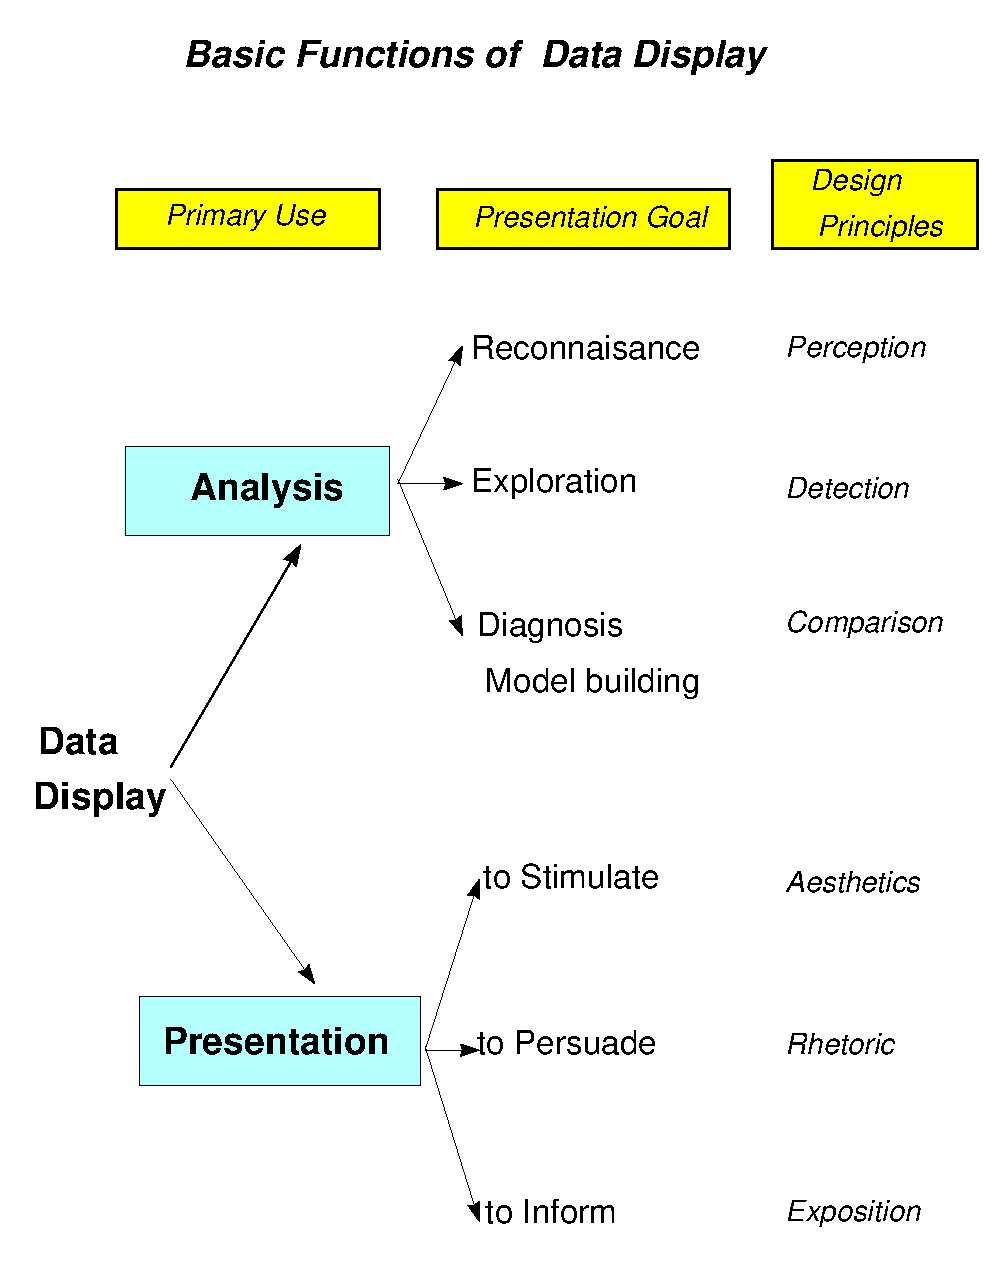
\includegraphics[scale=.8]{ch1/fig/datadisp}
  \caption[Basic functions of data display]{A taxonomy of the basic functions of data display by intended use and presentation goal}\label{fig:datadisp}
\end{figure}

The first distinction identifies \boldital{Analysis} or 
\boldital{Presentation} as the primary
communication goal of a data graphic
(with the understanding that a given graph may serve both purposes---or,
sadly, neither).

\subsubsection{Analysis graphs}
Graphs used for data analysis should clearly show the data, but they
should also ``force us to notice what we never
expected to see''
\cite[p. vi]{Tukey:77}.

Among graphical methods designed to help study or understand
a body of data, we may distinguish those designed for different
purposes.  As suggested in \figref{fig:datadisp}, each presentation goal
is associated with somewhat different design principles.
\begin{itemize}
\item \boldital{reconnaissance}---a preliminary examination, or an overview of a possibly complex terrain.
For this goal, we may be willing to sacrifice detail for a wider field of
view.
With a large, multi-way contingency table, for example, we might wish to
examine the collection of one-way and two-way marginal subtables
visually.  
\item \boldital{exploration}---graphs designed to help detect patterns or unusual
circumstances, or to suggest hypotheses, analyses or models.
For a binary response and a number of categorical or quantitative predictors,
a collection of smoothed plots of the response against each predictor
may suggest important variables to be included in a model,
extreme observations which should be examined, etc.
\item \boldital{diagnosis}---graphs designed to summarize or critique
a numerical statistical summary.
\end{itemize}

\subsubsection{Presentation graphs}
Presentation graphics have different goals as well.
We may wish to stimulate, or to persuade, or simply to inform.
As in writing, it is usually a good idea to know what it is you
want to say with a graph, and tailor its message to that goal.

It is often the case that a graph originally prepared as an aid
to data analysis can be transformed to one intended for presentation
by simple re-design.
Sometimes this entails removing detail useful for the analyst
but which may be detract from the major message;
sometimes this may involve adding titles or annotation to make the
message more immediately apparent.
In still other cases, we may decide to change the graphic format
to make visual comparisons easier for the intended audience.

For example, \figref{fig:glogist00} shows two views of the results
of fitting a logistic regression model to the arthritis treatment
data (described in \secref{sec:logist-qual}).
The left panel shows the observed (points) and predicted probabilities of
improvement ($\pm 1$ standard error, giving approximate 67\%
confidence intervals) in the form of a line graph.
The right panel shows a possible re-design of this graph for presentation
purposes.
%% two subfig side-by-side
\begin{figure}[htb]
 \begin{minipage}[c]{.49\linewidth}
  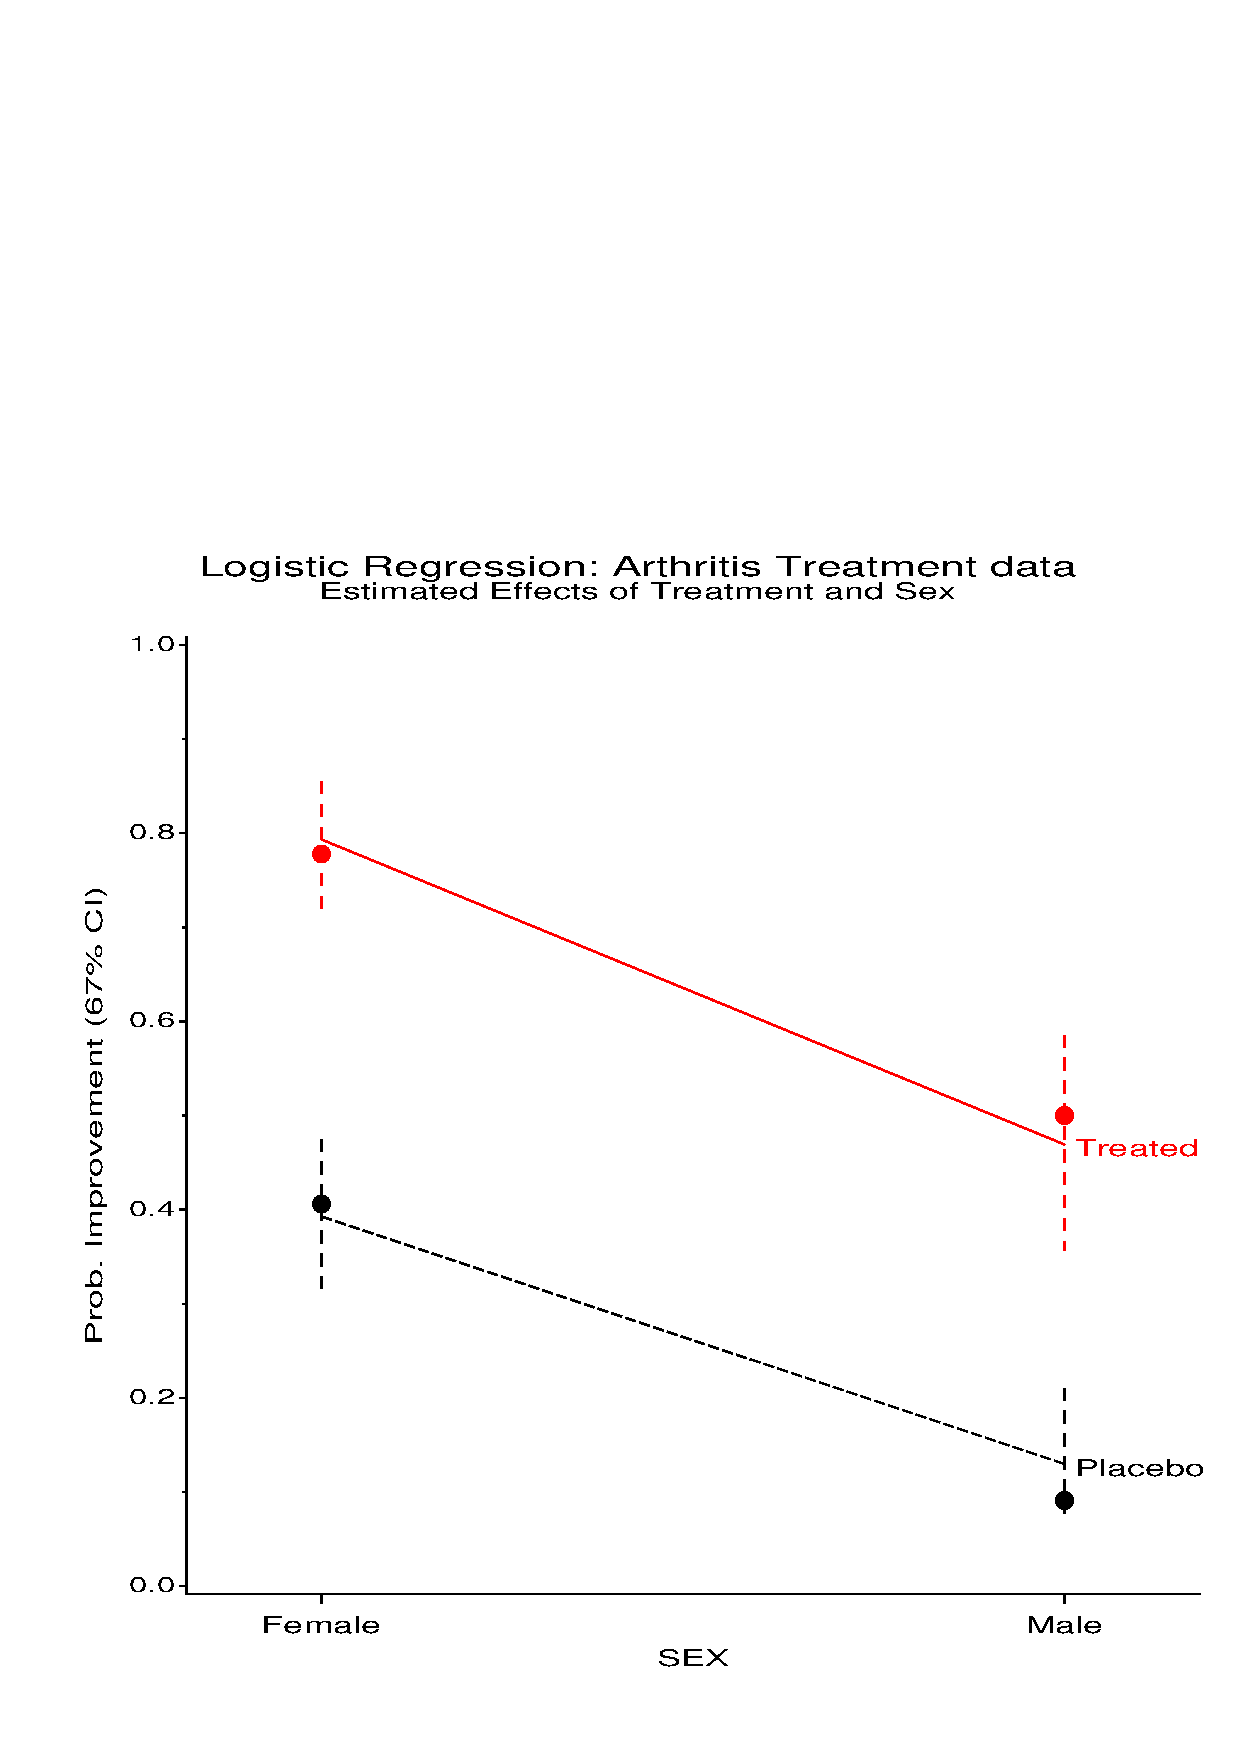
\includegraphics[width=1\linewidth]{ch6/fig/glogist11}
 \end{minipage}%
 \hfill
 \begin{minipage}[c]{.49\linewidth}
  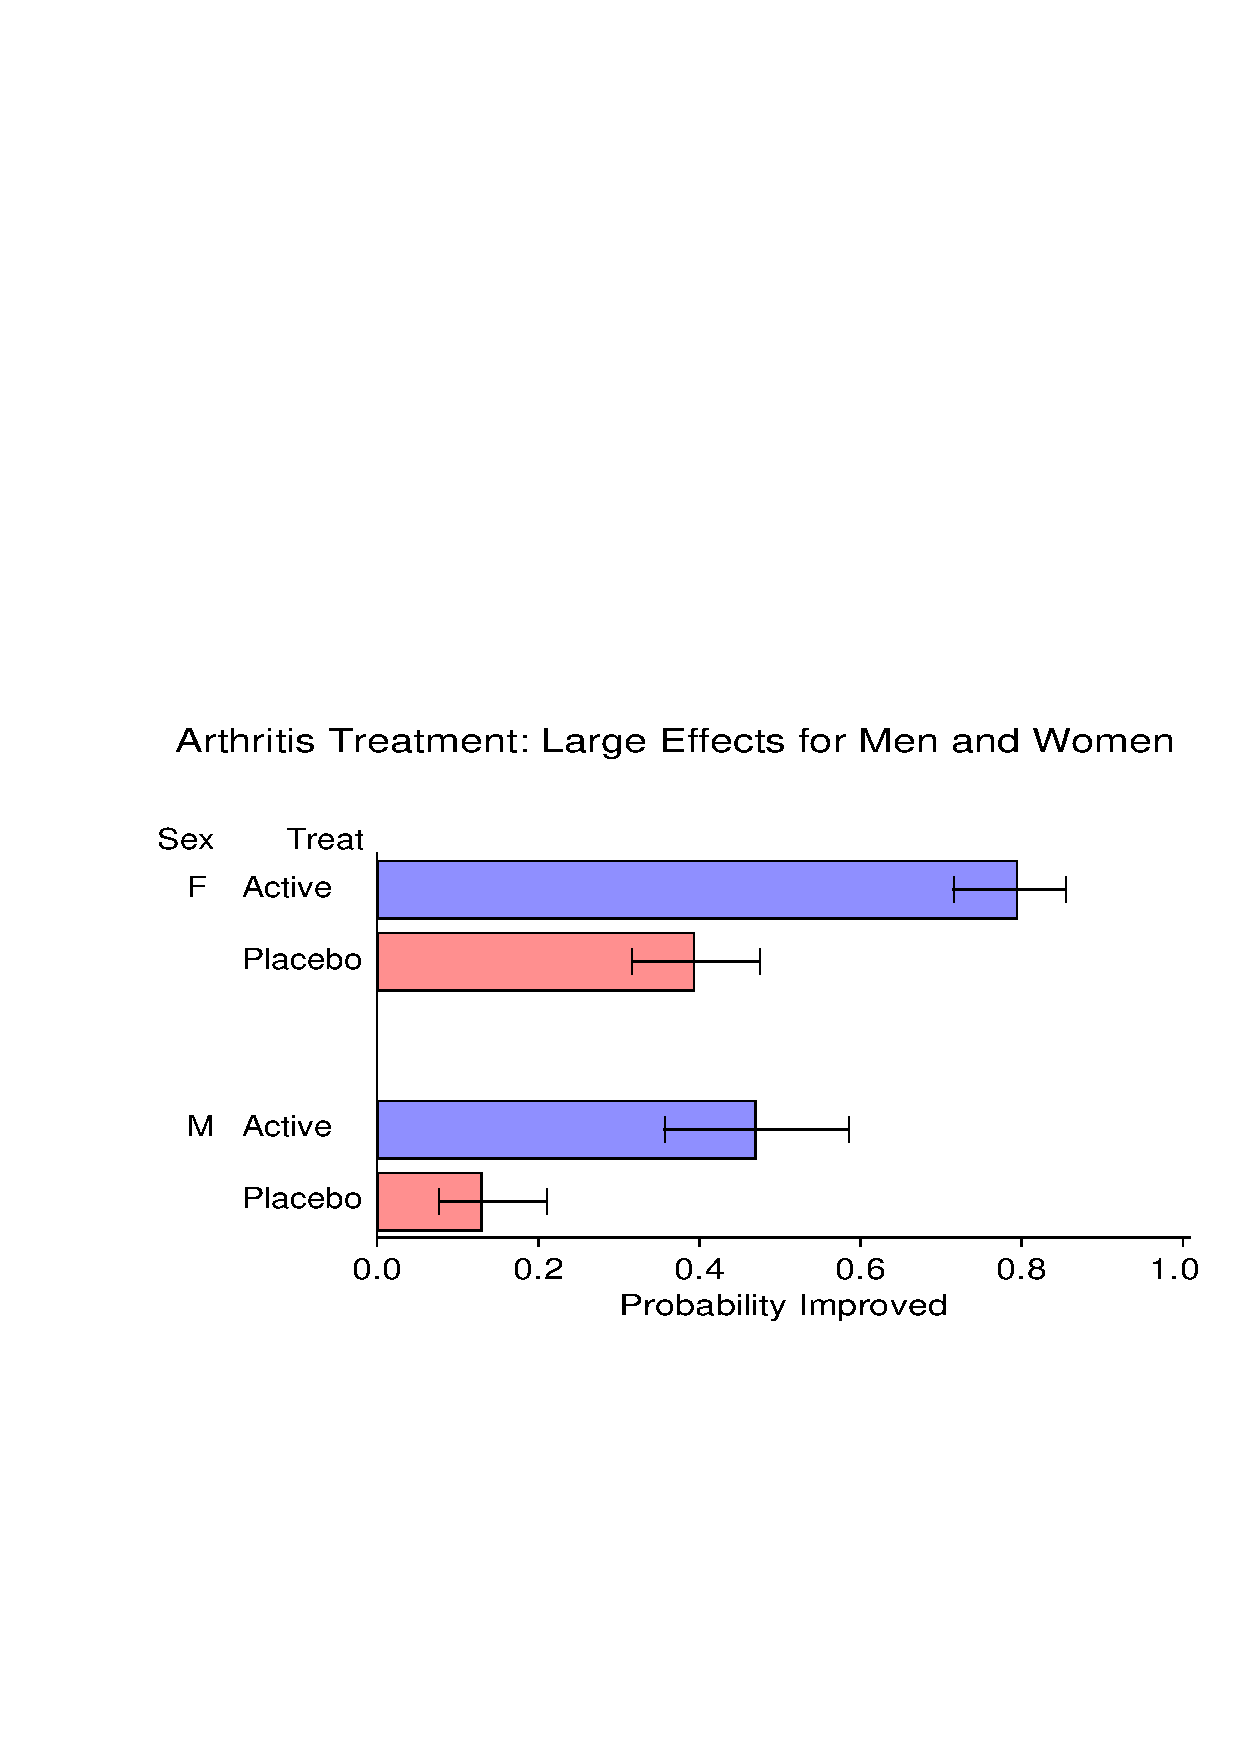
\includegraphics[width=1\linewidth,clip]{ch1/fig/glogist00}
 \end{minipage}
 \caption[Two graphical displays for arthritis treatment data]{Two graphical displays for arthritis treatment data. Left: initial analysis graph; right: re-design for presentation.}\label{fig:glogist00}
\end{figure}

The line graph might be preferred for analysis purposes, because it
shows
\begin{seriate}
\item the observed and fitted probabilities are quite similar,
\item there is a large effect of both treatment and sex, and
\item the effect of treatment is about the same for both men and women.
\end{seriate}
The presentation version contains the same predicted probabilities and error
bars as the original graph, but omits the observed probabilities
for simplicity.
The title explicitly
announces the conclusion to be drawn from the graph.


